\documentclass{sigchi}

% Remove or comment out these two lines for final version
\toappearbox{Woop woop woop!}
\pagenumbering{arabic}% Arabic page numbers for submission. 

% Use \toappear{...} to override the default ACM copyright statement (e.g. for preprints).

% Load basic packages
\usepackage{balance}  % to better equalize the last page
\usepackage{graphics} % for EPS, load graphicx instead
\usepackage{times}    % comment if you want LaTeX's default font
\usepackage{url}      % llt: nicely formatted URLs
\usepackage{framed}
\usepackage{mathtools}

% llt: Define a global style for URLs, rather that the default one
\makeatletter
\def\url@leostyle{%
  \@ifundefined{selectfont}{\def\UrlFont{\sf}}{\def\UrlFont{\small\bf\ttfamily}}}
\makeatother
\urlstyle{leo}


% To make various LaTeX processors do the right thing with page size.
\def\pprw{8.5in}
\def\pprh{11in}
\special{papersize=\pprw,\pprh}
\setlength{\paperwidth}{\pprw}
\setlength{\paperheight}{\pprh}
\setlength{\pdfpagewidth}{\pprw}
\setlength{\pdfpageheight}{\pprh}

% Make sure hyperref comes last of your loaded packages, 
% to give it a fighting chance of not being over-written, 
% since its job is to redefine many LaTeX commands.
\usepackage[pdftex]{hyperref}
\hypersetup{
pdftitle={SIGCHI Conference Proceedings Format},
pdfauthor={LaTeX},
pdfkeywords={SIGCHI, proceedings, archival format},
bookmarksnumbered,
pdfstartview={FitH},
colorlinks,
citecolor=black,
filecolor=black,
linkcolor=black,
urlcolor=black,
breaklinks=true,
}

% create a shortcut to typeset table headings
\newcommand\tabhead[1]{\small\textbf{#1}}


% End of preamble. Here it comes the document.
\begin{document}

\title{How Does My Audience Read My Visualization?}

% Note that submissions are blind, so author information should be omitted
\numberofauthors{1}
\author{
  \alignauthor Steve Rubin\\
    \affaddr{UC Berkeley, Computer Science Division}\\
    \affaddr{CS 294-10 -- Visualization Class Project}\\
    \email{srubin@cs.berkeley.edu}\\
}

% Teaser figure can go here
%\teaser{
%  \centering
%  
\includegraphics{Figure1}
%  \caption{Teaser Image}
%  \label{fig:teaser}
%}

\maketitle

\begin{abstract}
Abstract abstract abstract abstract.
\end{abstract}

\keywords{
  Visualization understanding; design
}

\category{H.5.m.}{Information Interfaces and Presentation (e.g. HCI)}{Miscellaneous
\\
}

\section{Introduction}

Research in information visualization and graphical perception has
often focused on creating effective visualizations for low-level
perception, such as ``what is the value represented by this bar in the
chart,'' and ``how much bigger is this bar than that bar.'' This work
is critical in gaining an understanding of which visual variables and
encodings are most easy to understand.

A parallel line of work has looked at how higher level attributes
affect the overall memorability of charts and graphs. This work aimed
to answer questions like, ``does chart junk make my graph easier to
remember,'' and ``what kinds of charts and graphs are most
memorable.''

While these two lines of work are posing interesting questions, they
neglect one of the most important goals of a visualization, which is
to convey a trend or a message to the viewer. The work on graphical
perception can tell us how to create the visualization so it is
legible, and the work on memorability can tell us how to spruce it up
so it sticks in the viewer's memory, but we are interested in learning
more about the how trends in a visualization strike a viewer as
important or unimportant. The ultimate vision of this line of research
is to take a designer's visualization, analyze it, and tell him
several key facts about the visualization, such as:

\begin{itemize}
  \item \textit{What trends do viewers think are most important?}
  \item \textit{How variable is the spread of trends that viewers
  think are important?}
  \item \textit{How well do the viewers' thoughts about this chart
  match the designer's intention?}
  \item \textit{What trends will the viewers retain after the
  visualization is taken away?}
\end{itemize}

In our methodology and system, a designer first creates a
visualization. This visualization is then posted to Amazon's
Mechanical Turk\footnote{\url{http://mturk.com}} where workers submit
what they think is the most important trend displayed in the
visualization. Simultaneously, the designer performs a nugget analysis
on the visualization, which amounts to them writing down the smallest
coherent trends that are found in the chart. The designer and his
colleagues assign ratings to the nuggets to get a score for each
nugget, ranging from 0 (true but unimportant) to 1 (vital importance).
The designer then reads the responses from Mechanical Turk, recording
the nuggets that are contained in each statement. Our system then
computes scores and aggregate statistics for the statements.

Ideally our system could performing the nugget assignment and analysis
in a fully automated way, but for this project we use a large amount
of manual identification and classification in the pipeline in order
to illustrate the potential benefits of such a system. The final
output of this system is a dashboard that shows some of the above key
facts to the designer of the visualization.

\section{Related Work}

This work touches on several areas of prior work from information
visualization as well as other subfields of computer science.

\subsection{Graphical Perception}

As the field of information visualization has matured over the years,
a large amount of research has studied how people view charts and
graphs at a perceptual level. In the foundational work on graphical
perception, Cleveland and McGill \cite{Cleveland1985, Cleveland1984}
performed experiments whose results found that some graphical
encodings were significantly easier for people to read and understand
than others. For example, they showed that estimating angles, as in
pie charts, is more error-prone than estimating positions, as in bar
or dot charts. Such guidelines are one type of deliverable in
graphical perception research. The other type are tools that automate
visualization creation given the guidelines we have learned from
experiments. While Cleveland's work gave generalized design principles
for creating charts and Mackinlay provided an automated presentation
tool \cite{Mackinlay1987}, our work focuses on the perceived
importance of trends in visualization rather than the viewer's ability
to accurately read the data.

\subsection{Memory}

Recent work in the computer vision community has explored the question
of ``What makes a picture memorable?''~\cite{isola2011makes}. This
work posed an image memory task to workers on Amazon's Mechanical Turk
and then learned predictors from image features to memorability. These
tasks were focused on the overall memorability of images, and not on
specific details of images. Later work took this methodology and
extended it to information visualizations~\cite{borkin2013makes}.
Because the methodology mirrored that of the earlier work on image
memorability, its results focused on overall memorability and not on
the memorability of specific trends in the visualization. Ultimately,
when a designer is creating a visualization, he likely wants to
communicate certain trends and ideas; getting the viewer to remember
exactly what the visualization looked like is a secondary concern. The
methodology used the measure the memorability of
visualizations~\cite{borkin2013makes} shows, as should be expected,
that charts with images (chart junk) and charts with atypical
structures (i.e., not a bar chart or a line chart, etc.) are more
memorable. In our work, we hope to uncover what viewers take away from
the visualization rather than just whether the chart made a visual
impression.

\subsection{Chart Junk}

The work on visualization memorability~\cite{borkin2013makes} showed
that charts containing images tend to be more memorable. Prior work
sought to quantify the ability of chart junk and visual embellishments
to aid in the memorability and understanding of a
chart~\cite{bateman2010useful}. This work suggested that, contrary to
advice given by thought-leaders in information
visualization~\cite{tufte1983visual}, charts with visual
embellishments gave viewers no worse accuracy in reading the data and
trend, and were easier to recall later on. Several sources have
pointed out numerous methodological issues with this
paper~\cite{Few,junkcharts}, so the question of the utility of chart
junk remains open to further research. While our work in its current
state does not specifically address the chart junk issue, our methods
and system could ultimately be used to study the effect of visual
embellishments on chart understanding.

\subsection{Crowdsourcing Data Analysis}

Our pipeline for learning what viewers understand about visualizations
relies, obviously, on the impression of viewers. This kind of data
could be collected in a lab study, but for the sake of future
scalability, we decided to deploy our visualizations to Mechanical
Turk. In running these tasks on Turk, we run the risk of getting noisy
data. However, we avoid this by using only workers in the United
States with at least a 95\% ``approved'' rating. Prior work in
crowdsourcing data analysis~\cite{willett2012strategies} describes
additional strategies we can employ to ensure high quality responses.

\subsection{Summarization evaluation}

Our analysis pipeline requires that we have way of taking a statement
from a user and somehow quantifying its ``goodness.'' This is an
inherently subjective problem, so we look to prior work in
summarization evaluation which shows a method for obtaining subjective
``goodness'' ratings for different facts about a subject by collecting
the ratings from multiple trusted colleagues and combining them into
final ratings~\cite{lin2006will}. This approach inspired our nugget
rating and assignment approach that we use in determining the worth of
each statement.

\section{Methods}

We want to discover what trends viewers think are important about a
visualization, the variability of the spread of trends that viewers
think are important, and how well the viewers' thoughts about the
chart reflect the designer's intention. To explain our methodology,
suppose that the designer has designed the chart that shows where gaps
have widened between whites and blacks in the past fifty years (Figure
\ref{fig:racialgaps}).

\begin{figure}[t]
  \begin{center}
    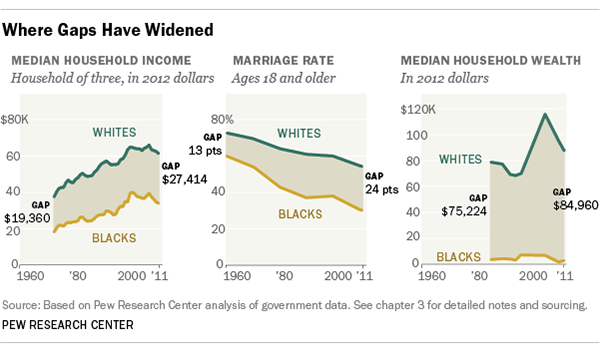
\includegraphics[width=3.33in]{figures/racialgaps.png}
  \end{center}
  \caption{A figure on racial gaps in the past 50 years, from Pew Research. We will use this visualization for our running example.}
  \label{fig:racialgaps}
\end{figure}

Our data collection and analysis pipeline contains steps that are
executed by the crowd, by the designer and his colleagues, and
automatically by our system. The full pipeline is shown in Figure
\ref{fig:pipeline}, and the following subsections will walk through
each phase of this pipeline.

\begin{figure}[t]
  \begin{center}
    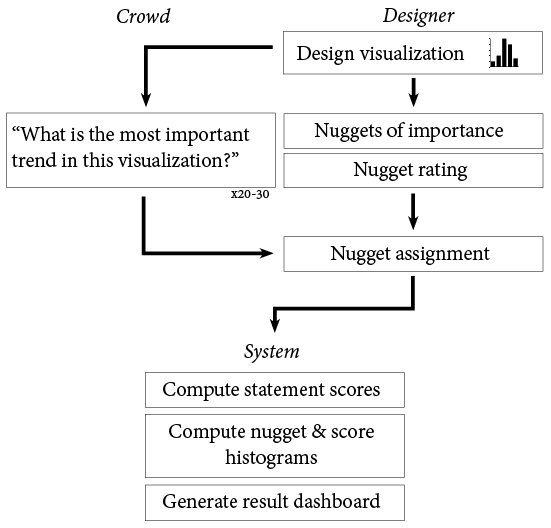
\includegraphics[width=3.33in]{figures/pipeline.png}
  \end{center}
  \caption{Our data collection and analysis pipeline.}
  \label{fig:pipeline}
\end{figure}

\subsection{Design}

The first stage of the pipeline is for the designer to create the
visualization. For this example, the designer creates the graph shown
in Figure \ref{fig:racialgaps}.

\subsection{Crowdsourcing}

\begin{figure}[t]
  \begin{framed}
  \begin{center}
    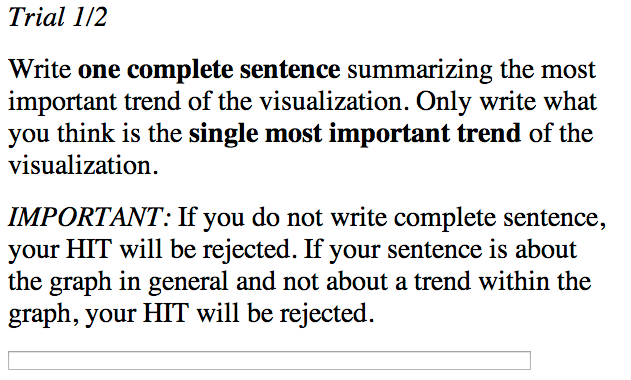
\includegraphics[width=3.33in]{figures/instrument.png}
  \end{center}
  \end{framed}
  \caption{An example of the survey instrument that is posted to Mechanical Turk. \textit{Note: the visualization itself is not shown in this figure to save space. In the real instrument, the visualization would appear above the text shown here.}}
  \label{fig:instrument}
\end{figure}

Once the designer has created the visualization, he pushes it to
Mechanical Turk. On Mechanical Turk, workers see a very simple task
that first walks them through a thorough set of instructions and
examples, and then asks them to write what they think is the single
most important trend of the visualization that they are viewing.
Figure \ref{fig:instrument} shows an example of our survey instrument.

We collect twenty to thirty statements for the visualization, but the
designer can collect as many or as few responses as he wants depending
on the complexity of the visualization, how confident the designer
wants to be of the analysis, and how much he wants to spend on crowd
workers.

We have built an extensive system for managing tasks on Mechanical
Turk that provides the designer with the following functionality:

\begin{itemize}
  \item \textbf{Multiple visualizations can be posted for analysis at once.}
  This allows the designer to offer a higher price for a batch of
  visualizations rather than a lower price for a single visualization.
  While this may seem trivial, workers on Mechanical Turk
  (particularly the high quality 95\% acceptance, US workers that we
  want) appear to be much quicker to accept a HIT offering fifty cents
  than one offering ten cents. This improves the rate in which the
  designer can collect data.
  \item \textbf{Workers will never see a visualization more than
  once.} This is crucial for maintaining the integrity of the
  collected data.
  \item \textbf{Multiple versions of a single visualization can be analyzed at
  once.} The system guarantees that no worker will see more than one
  version of the visualization. Again, this is crucial for maintaining
  integrity of the data. Our system can also accommodate the case
  where the designer \textit{wants} one person to see multiple
  versions of a visualization.
  \item \textbf{HITs can be re-posted without any negative
  consequence.} The state logic that dispatches tasks to workers is
  controlled by our server rather than on Mechanical Turk itself, so
  canceling and re-posting a HIT will not lose any state, but it will
  have the positive effect of bringing the HIT back to the top of the
  task list. This increases the visibility of the task, which improves
  the rate in which the designer can collect data.
  \item \textbf{New studies, instructions, and prompts can easily be
  added to the task management system.} While this is not particularly
  important in light of the pipeline presented in this work, it was
  critical in rapidly iterating on the study in order to get high
  quality feedback from crowd workers.
\end{itemize}

Our task management system can be used for any kind of study on
Mechanical Turk, not just the tasks described in this pipeline.

\begin{figure}[t]
  \begin{framed}
  \begin{center}
  \begin{enumerate}
    \item The gap in median household income, marriage rate, and
    median household wealth between whites and blacks have all grown.
    \item There is still a large financial gap between whites and blacks
    \item Trends are showing that whites income and wealth are increasing while black income and wealth remains relatively unchanged.
    \item The median household wealth for whites spiked much higher than blacks in the middle of the last decade.
    \item Between 1960 and 2012 the biggest gap between blacks and white has been shown in their median household wealth.
  \end{enumerate}
  \end{center}
  \end{framed}
  \caption{A sample of 5 responses ($n=30$) from crowd workers to the prompt, ``Write one complete sentence summarizing the most important trend of the visualization.''}
  \label{fig:sample}
\end{figure}

For our visualization (Figure \ref{fig:racialgaps}), Figure
\ref{fig:sample} shows 5 of the 30 responses we collected from crowd
workers. Notice that they have varying levels of ``goodness;'' for
example, statement 5 does not make sense because there is no notion of
what the ``biggest'' gap means because the three sub-charts of Figure
\ref{fig:racialgaps} have incomparable units and meanings.

\subsection{Nugget Analysis}

In parallel with the designer collecting data on Mechanical Turk, he
performs his own analysis on the visualization. The designer must
create a list of ``nuggets,'' which are small, ideally mutually
exclusive trends about the visualization. This is a manual process,
but it should not be difficult for the designer because we assume that
he had a good idea about \textit{why} he made the visualization in the
first place and knows what trends the visualization does and does not
show. Figure \ref{fig:nuggets} shows the list of nuggets that the
designer could create for our visualization. Note that the list of
nuggets does not necessarily need to contain every possible trend or
fact about the visualization; if the designer thinks a particular
trend has no importance, he can leave it off the list of nuggets.

\begin{figure}[t]
  \begin{framed}
  \begin{center}
    \begin{enumerate}
    \item Median household wealth for blacks has been relatively constant since 1960.
    \item Median household income has increased for whites and blacks since 1960.
    \item The gap in marriage rate between whites and blacks has grown between 1960 and 2011.
    \item Median household income spiked for whites in the 90's and early 2000's but has since dropped dramatically.
    \item Marriage rate has decreased for whites and blacks since 1960.
    \item Median household wealth isn't much different for whites or blacks than it was in 1960.
    \item The gap in household wealth between whites and blacks has grown between 1960 and 2011.
    \item Marriage rates have steadily decreased since 1960.
    \item The gap in median household income between whites and blacks has grown between 1960 and 2011.
    \item The gap between whites and blacks in median household wealth peaked in the mid 2000's.
    \item There exists a financial gap between blacks and whites.
    \end{enumerate}
  \end{center}
  \end{framed}
  \caption{Nuggets created by the designer for the chart in Figure \ref{fig:racialgaps}.}
  \label{fig:nuggets}
\end{figure}

This list of nuggets represents a set of potentially important
statements that can be made about the visualization. However, some of
these nuggets are likely more important than others. If the designer
has a strong sense of the relative importance of these nuggets, he
should assign each one a weight between 0.1 and 1.0 (here, 0 is
reserved for completely unimportant or wrong statements, so none of
the nuggets should have a weight of 0; more on this later).

In many cases, the designer may not be able to come up with these
weights on his own. There exist multiple reasons why this might
happen. For example, the designer might have a sense of what the few
most important points are, but may not know how to rank the other
statements. In this case, we propose a method of creating weights for
nuggets that draws on an idea from the text retrieval (TREC)
community~\cite{lin2006will}.

The designer selects $k-1$ colleagues that he trusts will be able to
properly understand the visualization. Then the designer and his
colleagues independently assign a rating of either 0 or 1 to each
nugget. Here, `1' means that the statement is vitally important,
whereas `0' means that the statement is correct, but not as important.
These ratings are given in the context of the visualization; that is,
the raters are rating the nuggets on how important the nuggets appear
to be in the given visualization. For example, nugget 11, ``There
exists a financial gap between blacks and whites'' may be a very
important trend in the global sense, but in the visualization, the
fact that certain gaps between blacks and whites are widening seems to
be more important.

If we start with $n$ nuggets, this procedure gives us a matrix
$n\times k$ matrix $N$ that contains 0/1 entries, with each column
representing a single person's ratings. To compute the weight $w_i$ of
nugget $i$, we take

\[w_i = \left( \frac{\sum_{j=1}^k N_{ij} }{\max_{s\in\{1,2,\dots,n\}} \sum_{j=1}^k N_{sj}} \right) .9 + .1 \]

This guarantees that the minimum weight is at least .1, and the
maximum weight is 1. The maximum weights needs to be 1 because later
on, we want to consider the best possible response from a crowd worker
to have score 1. Likewise, we want the worst possible response that
still contains a nugget to be .1. We want completely unimportant and
false statements to have a score of 0.

So, once our system has computed the weight vector $\mathbf{w} = [w_1,
w_2,\dots,w_n]$ our system can proceed in assigning scores to the
crowdsourced statements. First, the designer must analyze each
statement $r$ and create an indicator vector $\mathbf{\delta^r}$ where

\[\delta^r_i = \begin{dcases*}
    1 & : nugget $i$ appears in statement $r$\\
    0 & : nugget $i$ is not in statement $r$
    \end{dcases*}
\]

The score $s_r$ for statement $r$ is the computed as the weighted
average of the included nuggets:

\[s_r = \frac{\mathbf{w}^T\mathbf{\delta^r}}{\|\mathbf{\delta^r}\|_1}.
\]

Once again, notice that the best statements will have a score of 1,
false or completely unimportant statements will have a score of 0, and
responses that contain only unimportant nuggets will have a score of
.1.

Figure \ref{fig:scorecomp} shows the nugget assignment and score
computation of the first two statements from Figure \ref{fig:sample}.

\setcounter{MaxMatrixCols}{20}

\begin{figure}[t]
  \begin{framed}
    From $k=2$ raters, we had
    \[
    N = \begin{bmatrix}
    0 & 0 & 1 & 0 & 0 & 0 & 1 & 0 & 1 & 0 & 1 \\
    0 & 0 & 1 & 0 & 1 & 0 & 1 & 1 & 1 & 1 & 0
    \end{bmatrix}^T
    \]

    So the computed nuggets weights were:
    \[\mathbf{w}=\left[0.1,0.1,1.0,0.1,0.55,0.1,1.0,0.55,1.0,0.55,0.55\right]\]

    Sample of statements:
    \begin{enumerate}
    \item The gap in median household income, marriage rate, and
    median household wealth between whites and blacks have all grown.
    \begin{align*}
    \mathbf{\delta^1} &= \left[0,0,1,0,0,0,1,0,1,0,0\right]\\
    s_1 &= \frac{1 + 1 + 1}{1 + 1 + 1} = 1
    \end{align*}

    \item There is still a large financial gap between whites and blacks
    \begin{align*}
    \mathbf{\delta^2} &= \left[0,0,0,0,0,0,0,0,0,0,1\right]\\
    s_2 &= \frac{.55}{1} = .55
    \end{align*}
  \end{enumerate}

  \end{framed}
  \caption{Nugget assignment and score computation of a sample of crowdsourced importance statements.}
  \label{fig:scorecomp}
\end{figure}

\subsection{Dashboard Generation}

Once the nuggets have been assigned and the scores have been computed,
the final step is to convey this information the the designer. While
the designer has looked over each crowdsourced statement of importance
individually during the nugget assignment phase, the goal of our
system is to present the data in aggregate. Figure XX shows a
prototype dashboard for communicating the results to the designer.



\section{Results}

\section{Discussion}

\section{Future Work}

Automation on automation. NLP. Yeah.

% If you want to use smaller typesetting for the reference list,
% uncomment the following line:
% \small
\bibliographystyle{acm-sigchi}
\bibliography{project_report}
\end{document}
